\documentclass[11pt]{article}
\usepackage{graphics,epsfig,amsmath,amssymb}
\usepackage{epsf}
\usepackage{boxedminipage}
\usepackage{fullpage}
\usepackage{fancyheadings}
\usepackage{times}
\usepackage{amsmath}
\usepackage{ifthen}
%\usepackage{pseudocode}
\usepackage{psfrag}
\pagestyle{fancy}

\setlength{\topmargin}{.2in}
\setlength{\parindent}{0in}
\setlength{\parskip}{.15in}
\setlength{\footskip}{0.1in}

\newcounter{pctr}
\stepcounter{pctr}

\newcounter{partctr}

\newcommand{\ie}{{\em i.e.}}
\newcommand{\eg}{{\em e.g.}}

\newcommand{\ch}{\item {\bf True~~/~~False~~}}
\newcommand{\tfnote}{\probnote{Circle True or False for each choice.}}
\newcommand{\allapply}{\probnote{Circle ALL that apply}}
\newcommand{\bestanswer}{\probnote{Circle the BEST answer}}
\newcommand{\ansbelow}{\probnote{Answer legibly in the space below.}}

\renewcommand{\thesection}{{\bf\Roman{section}}}
\renewcommand{\theenumi}{{\bf\Alph{enumi}.}}
\renewcommand{\labelenumi}{{\bf\Alph{enumi}.}}

\newcommand{\setversion}[1]{\def\version{#1}}
\setversion{answers}
%\setversion{quiz}

\ifthenelse{\equal{\version}{answers}}{
    \newcommand{\sols}[1]{#1}
}{
    \newcommand{\sols}[1]{}
}


\begin{document}

\newcounter{answer}
\newenvironment{answer}[1][\relax]{\refstepcounter{answer}\begin{list}%
 {}{\leftmargin 0pt\rightmargin 0pt\labelsep 3pt\parsep 0pt%
 \setlength{\listparindent}{\parindent}}
    \item {\bf Answer \theanswer #1}\
    }{\hspace*{\fill}$\blacksquare$\end{list}} 



% uses these macros to delimit problems
\newcommand\prob[1]%
  {\begin{itemize}\item[]%
   \vspace{.2in}{\bf\thepctr. ~[#1~ points]:}\stepcounter{pctr}}
\newcommand\eprob{\end{itemize}}
\newcommand\probnote[1]%
  {\\\begin{tabular}{cr} \hspace{3in} & {\bf (#1)} \\ \end{tabular}}

% headers/footers
\lhead[\fancyplain{}{\bf Page \thepage ~of \pageref{lastpage}}]%
      {CS 6250 Fall 2011, Quiz 1}
\lfoot[{\bf Name: }]%
      {{\bf Name: }}
\rhead[CS 6250 Fall 2011, Quiz 1]%
      {\fancyplain{}{\bf Page \thepage ~of \pageref{lastpage}}}
\cfoot{}
%\setlength{\headrulewidth}{0in}
\setlength{\headsep}{.3in}

 % Compact itemize and enumerate.  Note that they use the same counters and
% symbols as the usual itemize and enumerate environments.
\def\compactify{\itemsep=0pt \topsep=0pt \partopsep=0pt \parsep=0pt}
\let\latexusecounter=\usecounter
\newenvironment{CompactItemize}
  {\def\usecounter{\compactify\latexusecounter}
   \begin{itemize}}
  {\end{itemize}\let\usecounter=\latexusecounter}
\newenvironment{CompactEnumerate}
  {\def\usecounter{\compactify\latexusecounter}
   \begin{enumerate}}
  {\end{enumerate}\let\usecounter=\latexusecounter}


\cfoot{}
\pagestyle{empty}

\begin{center}
\begin{tabular}{lr}
\resizebox{1in}{!}{
\includegraphics{GT}}
&
\parbox{4in}{
    {\Large\it College of Computing} \\ \\
    {\LARGE\sf Georgia Institute of Technology} 
}
%
\end{tabular}
\end{center}

\begin{center}
{\Large{\bf CS 6250: Computer Networking: Fall 2011} \\
 \vspace{.15in} \Huge{\bf Quiz I}} 
%\vspace{.2in}

% this is the box on the first page with overall quiz information
\begin{boxedminipage}[h]{6in}
There are \underline{13 questions} (and one bonus question) and
  \underline{\pageref{lastpage} pages} in this quiz booklet (including
  this page).  Answer each question according to the instructions given.
  You have {\bf 85 minutes}.

%\vspace{.1in} The last page is an easy question.  {\em Rip this
%page off of your exam for five bonus points.}  Turn it in anonymously if
%you like.


\vspace{.1in} 
If you find a question ambiguous, write down any
assumptions you make.  {\bf Be neat and legible.}  If I can't
understand your answer, I can't give you credit!  There are three pretty
challenging questions (clearly marked); you may want to look through the
whole quiz and save those for last.

\vspace{.1in} 
Use the empty sides of this booklet if you need scratch space.  You
may also use them for answers, although you shouldn't need to.  {\em If you
do use the blank sides for answers, make sure to clearly say so!}

\vspace{.1in} 
{\bf Note well: Write your name in the space below AND your initials at the bottom of each
page of this booklet.}

\begin{center}{\bf THIS IS AN ``OPEN NOTES, OPEN PAPERS'' QUIZ.\\
LAPTOPS ARE ALLOWED, BUT ONLY FOR REVIEWING PAPERS AND NOTES \\
NO OTHER MATERIALS, NO PHONES, NO PDAS.\\
{\em ABSOLUTELY NO EMAIL OR MESSAGING OF ANY KIND!} \\
MAKE SURE YOU'VE READ ALL THE INSTRUCTIONS ABOVE!}
\end{center}
{\em Initial here to indicate that (1)~you've read the instructions and (2)~
you agree to abide by the Georgia Tech Honor Code: }

\vspace{.1in} The last page has easy bonus questions, which you can
answer outside of the allotted time.  Rip the last page off of your
quiz for five bonus points.  Turn it in anonymously if you like.

\end{boxedminipage}
\end{center}
\vspace*{0.25in}
\begin{center}
{\it Do not write in the boxes below}
\end{center}

\begin{center}
\begin{tabular}{|l|l|l|l|l|l|l|l|l|} \hline \hline
{\bf 1-5 (xx/20)}& {\bf 6-10 (xx/30)}& {\bf 11-13 (xx/20)} &{\bf Bonus (5+xx)} & {\bf Total
  (xx/70)}  \\ \hline 
 & & & & \\ 
 & & & &\\ \hline \hline
\end{tabular}
\end{center}

\vspace{.2in}
{\bf\Large{Name:}}

\newpage
\pagestyle{fancy}

\section{Warmup}

\prob{4} Which of the following is true about static configuration
analysis (like the type in the {\em rcc} paper)?
\allapply

\setcounter{partctr}{0}
\begin{list}{\bf\Alph{partctr}.}{\usecounter{partctr}}
\item Static configuration analysis never raises false alarms; that is,
  if it detects an error, it is always correct.
\item Sometimes the behavior of routing protocols depends on route
  message ordering, so static configuration analysis cannot detect all
  errors. 
\item Static configuration analysis requires writing new tests for every
  routing protocol.
\item Data-plane analysis tools like Anteater often make it easier to
  understand how to correct a configuration error, since it checks the
  state of the data plane directly.
\item All of the above.
\end{list}
\eprob

\sols{
\begin{answer}
The answer is: (B), (C).
\end{answer}
}


\prob{4} Which of the following is true about S-BGP?
\allapply
\setcounter{partctr}{0}
\begin{list}{\bf\Alph{partctr}.}{\usecounter{partctr}}
%\begin{enumerate}
\item An S-BGP router signs the AS path including the {\em next} AS
  along the path, to prevent path shortening attacks.
\item S-BGP does not prevent an AS from falsely withdrawing a route
  advertisement. 
\item S-BGP guarantees that data packets travel along the advertised AS path
  to the destination.
\item S-BGP requires a certificate authority that maintains accurate
  mappings of each portion of IP address space and the AS that owns it.
\item None of the above.
\end{list}
\eprob

\sols{
\begin{answer}
The answer is: (A), (B), (D).
\end{answer}
}

\newpage
\prob{4} Which of the following most accurately describes the {\em most common}
uses for eBGP, iBGP, and IGP?
\bestanswer
\setcounter{partctr}{0}
\begin{list}{\bf\Alph{partctr}.}{\usecounter{partctr}}
%\begin{enumerate}
\item eBGP is used
  within an AS for external destinations, iBGP is used between ASes for
  external destinations, and IGP is used within an AS for internal destinations.
\item eBGP is used between ASes for external destinations, iBGP is used
  within an AS for external destinations, and IGP is used within an AS
  for destinations within an AS.
\item eBGP is used between ASes for external destinations, iBGP is used
  within an AS for internal destinations, and IGP is used within an AS
  for external destinations.
\item None of the above
\end{list}
\eprob

\sols{
\begin{answer}
The answer is (B).
\end{answer}
}

\prob{4} Which of the following is true about the Kapela attack on BGP?
\allapply
\setcounter{partctr}{0}
\begin{list}{\bf\Alph{partctr}.}{\usecounter{partctr}}
%\begin{enumerate}
\item The attack requires the attacker's neighboring AS to accept a
  route advertisement for a prefix that the attacker does not own.
\item The attack depends on AS ``sender-side loop detection'' (i.e.,
  checking the AS path for one's own AS before accepting the route). 
\item The victim might be able to discover the attack by noticing
  a change in end-to-end latency along the path.
\item The victim might be able to discover the attack using traceroute.
\item None of the above
\end{list}
\eprob

\sols{
\begin{answer}
The answer is: (A), (B), (C).
\end{answer}
}


\prob{4} Which of the following can an AS use in its route
advertisements to indicate to a neighboring ``backup'' upstream AS to
tell the backup AS to send it traffic through a different ``primary'' AS (as
opposed to sending it traffic directly)?  \allapply
\setcounter{partctr}{0}
\begin{list}{\bf\Alph{partctr}.}{\usecounter{partctr}}
%\begin{enumerate}
\item the BGP ``community'' attribute
\item Multiple exit discriminator
\item Local preference
\item AS path prepending
\item All of the above
\end{list}
\eprob

\sols{
\begin{answer}
The answer is: (A), (D).
\end{answer}
}




\newpage
\section{Potpourri}

\prob{5} In his paper, {\em The Design Philosophy of the DARPA Internet
  Protocols}, Clark explains how fate-sharing allows the network
architecture to survive failures.  (1)~Explain how storing connection state
information at end hosts constitutes fate sharing.  (2)~Does the 4D
architecture of separating the control plane from the data plane violate
fate sharing?  Why or why not? ~\ansbelow
%\vspace*{2.5in}
\eprob

\sols{
\begin{answer}
(1)~Storing connection state at end hosts constitutes fate sharing because
the state associated with the connection is only lost with the entities
associated with the connection itself (i.e., connection state is only
lost if a host fails). \\
(2)~It depends on where the state is stored.  All of the designs we
discussed in class do not violate fate sharing because the state
associated with forwarding traffic is still stored in the switches
themselves.  However, if the 4D controller stored some state that could
be lost during a failure that would prevent packet forwarding, then the
design could violate the fate sharing principle.
\end{answer}
}

\prob{3} Describe the {\em end-to-end argument}.  Give one example of a
network protocol or technology that violates the end-to-end argument
(and explain the violation).  ~\ansbelow 
%\vspace*{1.5in}
\eprob

\sols{
\begin{answer}
The end-to-end argument states that functions that can be implemented at
the ends of a connection should be implemented at the endpoints, rather
than at intermediate points between the endpoints.  The rationale for
this argument includes robustness and reliability, avoiding duplication
of function, and so forth.  One technology that violates the end-to-end
argument is NAT, because it involves keeping state about the connections
in the middle of the path.  Hop-by-hop congestion control is another
example of a violation.
\end{answer}
}


\newpage
\prob{6} Consider the AS graph below, which shows a set of ASes and
their business relationships.  Consider the following questions about
their relationships.
\begin{center}
\resizebox{0.5\textwidth}{!}{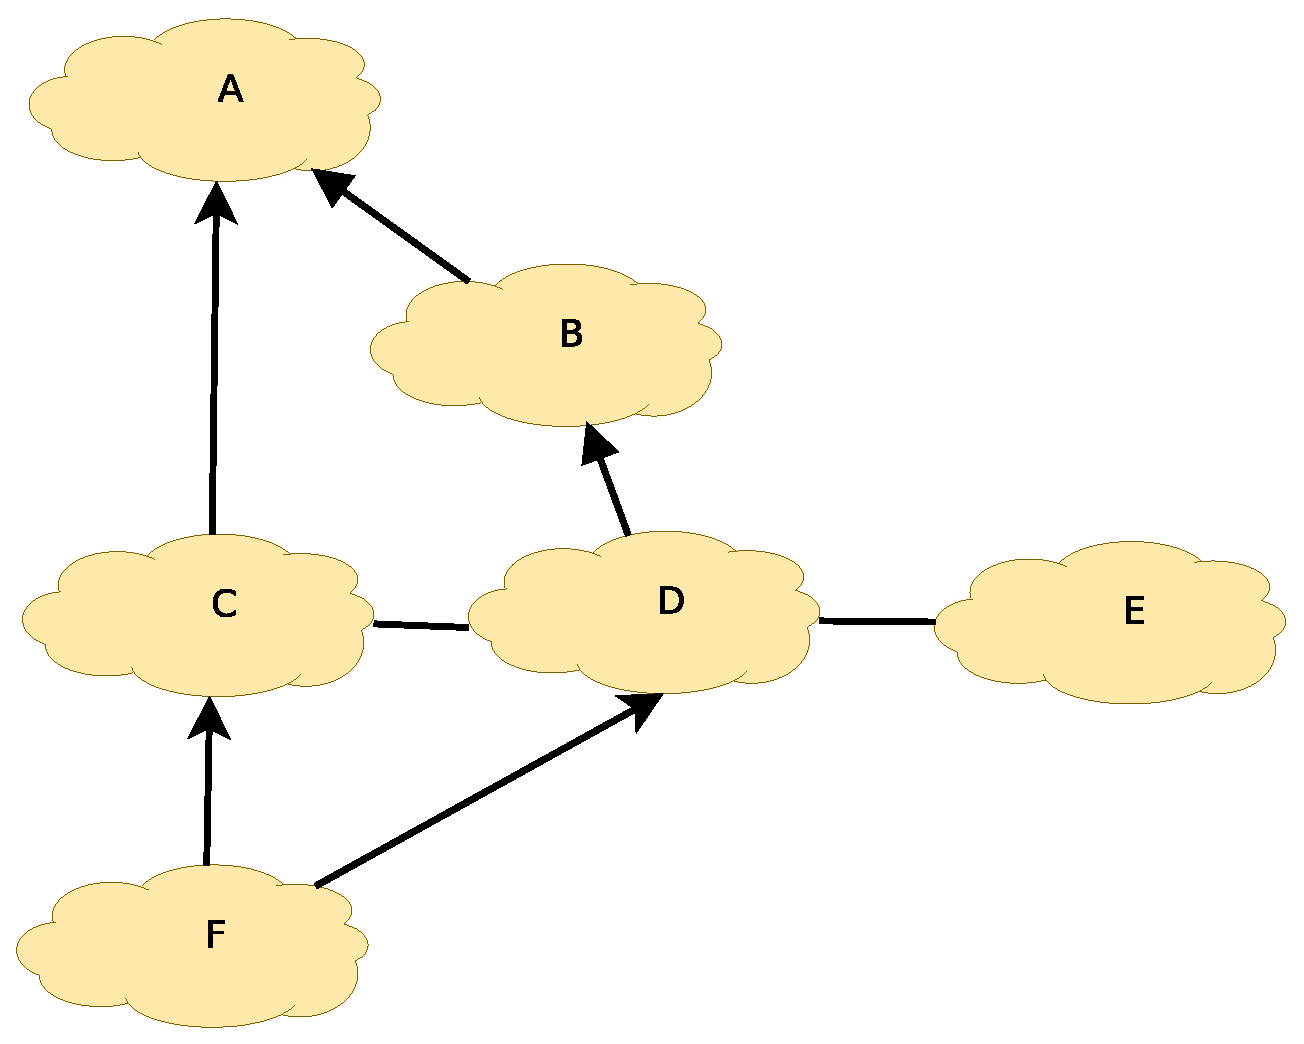
\includegraphics{bgp-as}}
\end{center}
\setcounter{partctr}{0}
\begin{list}{\bf\Alph{partctr}.}{\usecounter{partctr}}
\item Explain why, in the common case, the stub AS, $S$ would not readvertise
  routes it learned from provider $P1$ to its other provider, $P2$.
\item Explain why, in the common case, $P2$ would not readvertise routes
  that it learns from its peer $P1$ to its other peer, $P3$.
\item Describe a scenario involving ``regional peering'' where $P2$ might
  readvertise some of the routes that it learned from $P1$ to
  $P3$. State specifically which set of routes it might readvertise.
\end{list}
~\ansbelow 
%\vspace{2in}
\eprob

\sols{
\begin{answer}
In the common case, a stub AS would not readvertise routes it learned
from provider $P1$ to provider $P2$ because it pays for connectivity
from both providers, regardless of the direction of traffic flow.  For
a similar reason, routes are not advertised between peers: $P3$ is not
paying $P2$ to carry traffic for it to $P1$; doing so effectively incurs
$P2$ some cost (e.g., more traffic on its peering connection, which
could disrupt peering ratios, etc.).  Suppose that $P1$ and $P3$ need
connectivity to one another but do not have connectivity in the same
city: they might ask $P2$ to provide connectivity between each other's
customers, but only for prefixes in a particular city.
\end{answer}
}

\newpage
\prob{8} Consider the router backplane below, with packets arriving as
shown.  The number on each packet designates its intended output port.
Suppose that each input and output port have a rate of 1 Gigabit per
second. 
\begin{center}
\resizebox{0.5\textwidth}{!}{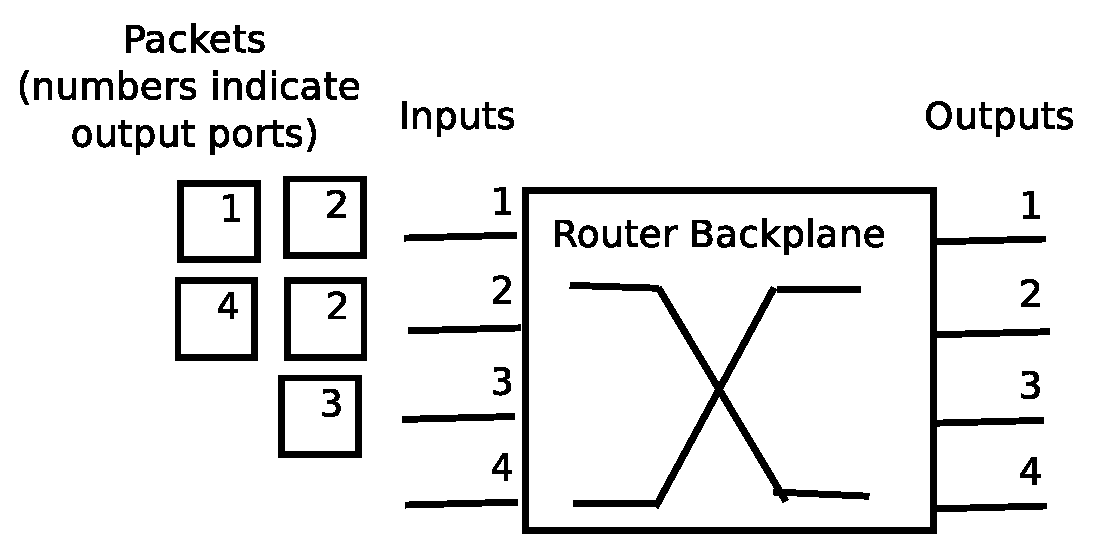
\includegraphics{backplane}}
\end{center}
\setcounter{partctr}{0}
\begin{list}{\bf\Alph{partctr}.}{\usecounter{partctr}}
\item Suppose the router has a {\em bus backplane} with throughput of 2
  Gigabits per second.  What is the total maximum throughput that the
  router can achieve? 
\item The example shows an example of head-of-line blocking.  Explain
  why, and explain how virtual output queueing can fix the problem.
\item Now suppose the router has a {\em crossbar switch backplane} with
  a throughput of 2 Gigabits per second (a ``speedup'' of 2) and virtual
  output queueing.  Given the packet arrival pattern shown in the
  figure, give a sequence of matchings of input ports to output ports
  that results in 100\% utilization (to save time, simple notation like
  ``Round 1: $1\rightarrow 2$'' is sufficient to indicate that you match
  input one to output two in round one).
\end{list}
~\ansbelow
\eprob

\sols{
\begin{answer}
The first question is a bit of a trick question: The total maximum
throughput is 1 Gigabit per second: only one input and output port can
be occupied on a {\em bus} for any given timeslot, so no parallelization
is possible. Head-of-line blocking exists in this case because inputs 1
and 2 both have packets destined for output 2; however, in a crossbar
backplane, either input 1 or input 2 could be matched to output 2 or
output 4, respectively.  A matching that could achieve 100\% utilization
is: round 1: $1 \rightarrow 2$, $2\rightarrow 4$, $3 \rightarrow 3$,
round 2: $1 \rightarrow 1$, $2\rightarrow 2$.
\end{answer}
}

\newpage
\prob{8} Consider the CDF below, which shows the distribution of IS-IS
failure durations in the a large IP backbone network over a four-month
period.   
\begin{center}
\resizebox{0.5\textwidth}{!}{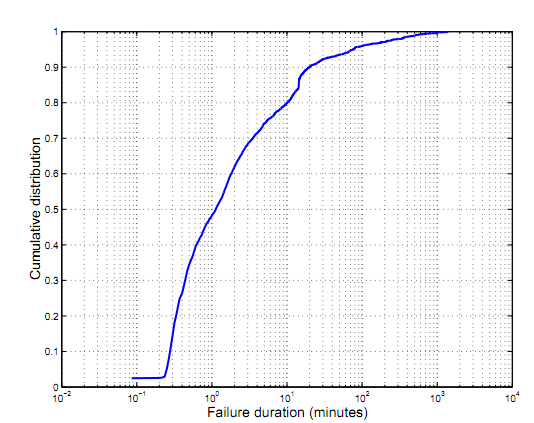
\includegraphics{isis-cdf}}
\end{center}
\setcounter{partctr}{0}
\begin{list}{\bf\Alph{partctr}.}{\usecounter{partctr}}
\item What is the median failure duration?
\item About what fraction of failures last longer than 20 minutes?  What
  is one possible cause of the failures that last longer than 20 minutes?
\item From Problem Set~1 (where you were asked about systems for
  measuring IS-IS traces), how were these measurements likely collected?
\item Paxson's paper {\em Strategies for Sound Internet Measurement}
  suggests cross-validation of measurements as a means for
  sanity-checking measurement results.  Describe one source of
  inaccuracy for the measurements below, and one way to
  cross-validate the measurements.
\end{list}
~\ansbelow 
\eprob

\sols{
\begin{answer}
The median failure duration is about 1 minute.  About 10\% of the
failures last longer than 20 minutes; one likely cause for these
long-lived outages is fiber cuts.  These measurements were likely
collected using an IS-IS ``monitor''---since IS-IS is a link-state
protocol that is flooded, a single monitor on the network would be able
to hear all link-state announcements.  One possible source of inaccuracy
might be timing syncrhonization problems that might result from the fact
that the LSAs are only captured from one place in the network.  Possible
ways of cross-validating these failure durations might be inserting a
second IS-IS monitor at a different place in the network, or using a
different technique altogether (e.g., probing in the data plane, using
traceroute, etc.)
\end{answer}
}


\newpage
\section{Measuring Broadband Access Networks}

\prob{6} The output below shows Netalyzr's measurements of buffering on
an access link.  
\begin{center}
\resizebox{0.75\textwidth}{!}{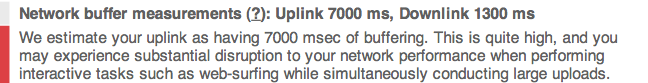
\includegraphics{netalyzr-buffer}}
\end{center}
\setcounter{partctr}{0}
\begin{list}{\bf\Alph{partctr}.}{\usecounter{partctr}}
\item Suppose that the {\em uplink} bandwidth on this access link is
  500~kilobits per second.  Compute the amount of buffering on the
  access {\em uplink}, in bytes.
\item Where might this buffering be occurring?
\item Explain how this amount of buffering might cause TCP senders to
  send at rates that are too high for the access link.
\end{list}
~\ansbelow
\eprob

\sols{
\begin{answer}
The amount of buffering is 500 kbits/second $\cdot$ 7 seconds $\cdot$ 1/8
bytes/bit: 437.5 kbytes.  This buffering is
likely occurring at the bottleneck link along the path, which is the
access network uplink in this case.  This amount of buffering slows
feedback to TCP senders because they will receive information about lost
packets much later than they would without buffering; as a result, a TCP
sender could open up its TCP window far too much before seeing the first
packet loss.
\end{answer}
}

\newpage
\prob{6} The traceroute below shows the output of a traceroute from the
Netalyzr servers back to a home access network that was running the
Netalyzr tool.   
\begin{center}
\resizebox{0.75\textwidth}{!}{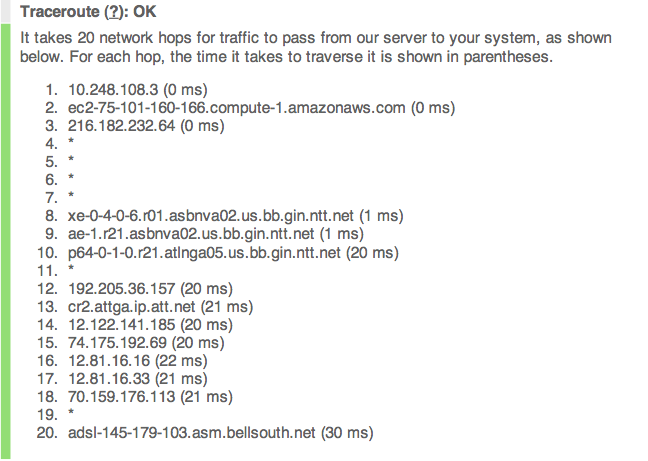
\includegraphics{netalyzr-traceroute}}
\end{center}
\setcounter{partctr}{0}
\begin{list}{\bf\Alph{partctr}.}{\usecounter{partctr}}
\item Why are there lines in the traceroute that list ``*''?
\item Give one reason why the hops shown might not be the same hops as
  the path that data packets actually travel.
\item Using your knowledge from the {\em 50 Gbps Router} paper about
  packet processing, give one reason why the time shown might be
  inaccurate.
\end{list}
~\ansbelow 
\eprob

\sols{
\begin{answer}
The lines in the traceroute with ``*'' are simply cases for which a
TTL-limited UDP probe never saw a time exceeded message.  This could be
caused by a number of factors: a lost UDP probe, a lost time exceeded
message on the reverse path, a firewall along the reverse path blocking ICMP
messages, etc.  As discussed in lecture, two reasons why the hops shown
might not be the same hops as the path that data packets travel is: (1)
load balancers can send packets along different paths, depending on
things like the destination port; (2) the IP address may be the source
IP address of the time exceeded message, depending on the
implementation.  Because ICMP is processed on the router's slow path (as
discussed in the referenced paper), the times reported by traceroute may
be inaccurate.
\end{answer} 
}

\newpage
\prob{8} George Burdell remembers from CS~6250 lecture that traceroute
discovers paths by sending UDP packets by incrementing the destination
port on each TTL-limited UDP packet.  
\setcounter{partctr}{0}
\begin{list}{\bf\Alph{partctr}.}{\usecounter{partctr}}
\item Why does traceroute increment the destination port on each UDP packet?
\item George observes: ``Incrementing the destination
port on each outgoing packet could cause a firewall or intrusion
detection system to raise an alarm.''  Is he right?  Why or why not?
\item George also observes: ``Incrementing the destination port on each
  outgoing packet could cause load balancers along the path to send each
  probe packet along a different path.''  Is he right?  Why or why not?
\item What fields in the UDP header might you be able to use for
  traceroute probes that would be guaranteed not to trigger load
  balancers or firewalls?
\end{list}
~\ansbelow 
\eprob

\sols{
\begin{answer}
Some implementations of traceroute increment the destiantion port on
each UDP packet because the ICMP time exceeded message that the router
returns must be matched to the appropriate hop; that time exceeded
message is returned with a portion of the original packet header.
Incrementing the destination port allows the header for each UDP probe
to be unique.  This can sometimes trip firewalls, since sending packets
with sequentially increasing port numbers can look like a ``port
scan''.  It can also cause load balancers to send each probe packet
along a different path, since many load balancers use a 5-tuple
(src/dest IP and port, plus protocol) to load balance along equal-cost
paths.  Other tools, such as Paris traceroute, use the checksum as a
unique identifier, rather than the 5-tuple (Paris traceroute was not
presented in class, but this question was mainly to see what you could
think of; many answers are acceptable for part D.).
\end{answer}
}

\newpage
\prob{6} {\bf Bonus.} Suppose that you would like to measure the
downstream throughput for an access link for which you do not have
direct access.  You have access to servers on the Internet and can ``ping''
the router that is on the downstream side of the access link, but you
don't have direct access to either the router, or any devices downstream
from the access router.  Design a probing scheme that you could send
from servers on the Internet to estimate the downstream throughput of
the access link.  State your assumptions and possible sources of inaccuracy.
~\ansbelow 
\eprob

\sols{ One possibility would be to send giant TCP ACK packets to each
  host/router on the other side of the access link; the host/router
  should respond with a small TCP RST packet.  In this way, the probing
  method could saturate the downstream link without saturating the
  upstream link.  If you are curious, this method and others are
  described in some detail in {\em Characterizing Residential Broadband
    Networks}, by Dischinger {\em et al.}.  }

\newpage
\section{Bonus: Anonymous Course Feedback}

{\bf This page is anonymous.}  Rip this off from your exam, and turn it
in separately if you like.  You'll get five points for simply ripping
off the last page of the exam, but I'd prefer if you fill it out and
hand it in in a separate stack.
\vspace{.5in}

What are the things you like most about the course so far?  Anything is
fair game here (topics, course structure, board technique, etc.).
\vspace{1.5in}


What are the things you like least about the course so far?  Again,
anything is fair game.
\vspace{1in}


What topics would you like to see covered?
\vspace{1in}




\label{lastpage}
\end{document}
